\chapter{Synchronization (Carrier, Timing, Frame)}
\label{ch:synchronization}

\begin{nontechnical}
\textbf{Synchronization is like tuning a radio perfectly}---the receiver must match the transmitter's frequency, phase, and timing, or you just hear noise!

\textbf{Think of it like dancing:}
\begin{itemize}
\item \textbf{Frequency sync:} Both partners dancing to the same music tempo
\item \textbf{Phase sync:} Both partners in step (not one ahead/behind)
\item \textbf{Timing sync:} Knowing when to start each move
\item \textbf{Frame sync:} Knowing when the song begins and ends
\end{itemize}

\textbf{Why it matters:} Your WiFi, GPS, and cell phone all spend milliseconds synchronizing before transmitting data. Without perfect sync, the signal is gibberish!
\end{nontechnical}

\section{Overview}

\textbf{Synchronization} is the process of aligning the receiver with the transmitter in frequency, phase, timing, and frame boundaries. It is critical for coherent demodulation and reliable data recovery.

\begin{keyconcept}
Without proper synchronization, even a perfectly received signal cannot be demodulated. \textbf{Synchronization is as critical as the modulation scheme itself}---failure in any of the four synchronization types (frequency, phase, timing, frame) results in complete data loss.
\end{keyconcept}

Synchronization forms the foundation for coherent detection and enables the receiver to extract information from the transmitted waveform.

\subsection{Four Types of Synchronization}

\textbf{1. Carrier Frequency Synchronization:} Match the receiver local oscillator frequency to the transmitter carrier frequency.

\textbf{2. Carrier Phase Synchronization:} Align the receiver carrier phase with the transmitter phase reference ($0°$).

\textbf{3. Symbol Timing Synchronization:} Sample received waveform at optimal instants (peak of matched filter output).

\textbf{4. Frame Synchronization:} Identify packet/frame boundaries in the continuous symbol stream.

\subsection{Consequences of Synchronization Errors}

\begin{itemize}
\item \textbf{Frequency offset:} Constellation rotation, inter-carrier interference (OFDM)
\item \textbf{Phase error:} Constellation rotation, increased BER
\item \textbf{Timing error:} Inter-symbol interference (ISI), suboptimal sampling
\item \textbf{Frame misalignment:} Lost packets, header decoding failure
\end{itemize}

\section{Mathematical Description}

\subsection{Carrier Frequency Offset (CFO)}

Carrier frequency offset arises from local oscillator (LO) frequency mismatch between transmitter and receiver:
\begin{equation}
\Delta f = f_{\text{LO,RX}} - f_{\text{LO,TX}}
\end{equation}
where:
\begin{itemize}
\item $\Delta f$ = carrier frequency offset (Hz)
\item $f_{\text{LO,RX}}$ = receiver local oscillator frequency
\item $f_{\text{LO,TX}}$ = transmitter carrier frequency
\end{itemize}

\textbf{Effect on received signal:}
\begin{equation}
r(t) = s(t) e^{j 2\pi \Delta f t} + n(t)
\end{equation}
where:
\begin{itemize}
\item $r(t)$ = received complex baseband signal
\item $s(t)$ = transmitted signal
\item $n(t)$ = additive noise
\end{itemize}

\subsection{Normalized CFO and Its Effects}

The \textbf{normalized CFO} is expressed as a fraction of the symbol rate:
\begin{equation}
\epsilon = \Delta f \cdot T_s = \frac{\Delta f}{R_s}
\end{equation}
where:
\begin{itemize}
\item $\epsilon$ = normalized carrier frequency offset (dimensionless)
\item $T_s$ = symbol period (seconds)
\item $R_s$ = symbol rate (symbols/second)
\end{itemize}

\textbf{Effect 1: Constellation rotation.} Phase advances by $2\pi\epsilon$ per symbol:
\begin{equation}
\phi_n = 2\pi\epsilon \cdot n
\end{equation}
where $n$ is the symbol index.

\textbf{Effect 2: Inter-carrier interference (ICI) in OFDM.} Subcarriers leak into adjacent carriers, degrading orthogonality.

\textbf{Effect 3: SNR degradation.} Effective SNR loss approximated by:
\begin{equation}
\text{SNR}_{\text{loss}} \approx 10 \log_{10}(1 + \text{SNR} \cdot (2\pi\epsilon)^2) \quad \text{dB}
\end{equation}

\begin{calloutbox}{Example: WiFi at 2.4 GHz}
Consider a WiFi system with $\pm 20$~ppm crystal oscillator tolerance:
\begin{itemize}
\item Carrier frequency: $f_c = 2.4$~GHz
\item CFO: $\Delta f = \pm 2.4 \times 10^9 \times 20 \times 10^{-6} = \pm 48$~kHz
\item Symbol rate: $R_s = 250$~ksps (OFDM subcarrier spacing)
\item Normalized CFO: $\epsilon = \pm 48{,}000 / 250{,}000 = \pm 0.192$ (19\%!)
\end{itemize}
\textbf{Conclusion:} CFO must be corrected before demodulation to avoid severe ICI.
\end{calloutbox}

\section{CFO Estimation Methods}

\subsection{Data-Aided (Preamble-Based) CFO Estimation}

Transmit known symbols (preamble, pilot tones) and correlate received signal with expected pattern:
\begin{equation}
\hat{\Delta f} = \frac{1}{2\pi T} \angle \left(\sum_{k=0}^{L-1} r_k \cdot s_k^*\right)
\end{equation}
where:
\begin{itemize}
\item $\hat{\Delta f}$ = estimated carrier frequency offset (Hz)
\item $r_k$ = received preamble symbol $k$
\item $s_k$ = known preamble symbol $k$
\item $L$ = preamble length (symbols)
\item $T$ = symbol period (seconds)
\end{itemize}

\textbf{Estimation range:} $|\Delta f| < \frac{1}{2T}$ due to phase ambiguity.

\textbf{Typical accuracy:} $\sim 10^{-4}$ of symbol rate in moderate SNR.

\subsection{Blind (Non-Data-Aided) CFO Estimation}

Blind methods exploit signal properties without requiring known preambles.

\textbf{Example for M-PSK:} Raise signal to $M$-th power to remove data modulation:
\begin{equation}
\hat{\Delta f} = \frac{1}{2\pi M T} \angle \left(\sum_{k=0}^{N-1} r_k^M\right)
\end{equation}
where:
\begin{itemize}
\item $M$ = modulation order (e.g., $M=4$ for QPSK)
\item $r_k$ = received symbol $k$
\item $N$ = number of symbols used for estimation
\end{itemize}

\textbf{Estimation range:} $|\Delta f| < \frac{1}{2MT}$ (reduced compared to data-aided).

\textbf{Advantage:} No preamble overhead.

\textbf{Disadvantage:} Reduced estimation range and accuracy compared to data-aided methods.

\subsection{Two-Stage Acquisition}

Practical systems use a two-stage approach combining wide-range coarse acquisition with high-accuracy fine tracking.

\textbf{Stage 1---Coarse acquisition:}
\begin{itemize}
\item Range: $\pm 50\%$ of symbol rate
\item Method: Preamble autocorrelation
\item Speed: Fast (few symbol periods)
\end{itemize}

\textbf{Stage 2---Fine tracking:}
\begin{itemize}
\item Accuracy: $\pm 0.1\%$ of symbol rate
\item Method: PLL or decision-directed feedback
\item Speed: Slower convergence
\end{itemize}

\begin{calloutbox}{Example: WiFi 802.11a}
WiFi uses dual preambles for two-stage synchronization:
\begin{itemize}
\item \textbf{Short preamble:} Coarse CFO estimation ($\pm 100$~kHz range)
\item \textbf{Long preamble:} Fine CFO estimation ($\pm 1$~kHz accuracy)
\end{itemize}
Total synchronization time: $\sim 16~\mu$s before data transmission begins.
\end{calloutbox}

\subsection{CFO Correction}

Once estimated, CFO can be corrected digitally or through analog frequency control.

\textbf{Digital correction} (post-downconversion):
\begin{equation}
r_{\text{corrected}}[n] = r[n] \cdot e^{-j 2\pi \hat{\epsilon} n}
\end{equation}
where:
\begin{itemize}
\item $r[n]$ = received baseband sample $n$
\item $\hat{\epsilon}$ = estimated normalized CFO
\item $r_{\text{corrected}}[n]$ = frequency-corrected signal
\end{itemize}

\textbf{Analog correction:} Adjust voltage-controlled oscillator (VCO) frequency using automatic frequency control (AFC).

\textbf{Hybrid approach:} Coarse analog correction followed by fine digital correction provides best performance with reduced computational complexity.

\section{Carrier Phase Synchronization}

\subsection{Phase Offset}

After CFO correction, a residual phase error $\theta$ remains:
\begin{equation}
r(t) = s(t) e^{j\theta} + n(t)
\end{equation}
where:
\begin{itemize}
\item $\theta$ = carrier phase offset (radians)
\item $s(t)$ = transmitted signal
\item $r(t)$ = received signal
\end{itemize}

\textbf{Effect:} The entire constellation rotates by angle $\theta$.

\subsection{Phase Error Tolerance by Modulation}

Different modulation schemes have varying tolerance to phase errors:

\begin{center}
\begin{tabular}{@{}lc@{}}
\toprule
\textbf{Modulation} & \textbf{Phase Tolerance} \\
\midrule
BPSK & $\pm 90°$ \\
QPSK & $\pm 45°$ \\
8-PSK & $\pm 22.5°$ \\
16-QAM & $\pm 11.25°$ \\
64-QAM & $\pm 3.75°$ \\
256-QAM & $\pm 2.8°$ \\
\bottomrule
\end{tabular}
\end{center}

\begin{warningbox}
Higher-order modulation schemes (e.g., 256-QAM) are extremely sensitive to phase errors. A phase error of just $\pm 2.8°$ causes constellation points to cross decision boundaries, resulting in symbol errors. This demands highly accurate phase tracking.
\end{warningbox}

\subsection{Phase-Locked Loop (PLL)}

The \textbf{phase-locked loop} is the classic analog/digital feedback system for carrier phase tracking.

\subsubsection{PLL Block Diagram}

\begin{center}
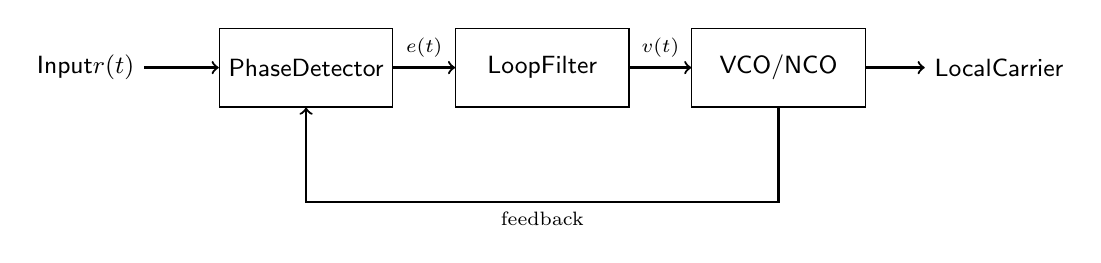
\begin{tikzpicture}[
  block/.style={rectangle, draw, minimum width=2.2cm, minimum height=1cm, font=\sffamily\small},
  node distance=2.5cm,
  font=\small
]
\node (input) {\sffamily Input\\$r(t)$};
\node[block, right of=input, node distance=2.8cm] (pd) {Phase\\Detector};
\node[block, right of=pd, node distance=3cm] (lf) {Loop\\Filter};
\node[block, right of=lf, node distance=3cm] (vco) {VCO/\\NCO};
\node[right of=vco, node distance=2.8cm] (output) {\sffamily Local\\Carrier};

% Forward path
\draw[->,thick] (input) -- (pd);
\draw[->,thick] (pd) -- node[above] {\scriptsize $e(t)$} (lf);
\draw[->,thick] (lf) -- node[above] {\scriptsize $v(t)$} (vco);
\draw[->,thick] (vco) -- (output);

% Feedback path
\draw[->,thick] (vco.south) -- ++(0,-1.2) -| node[near start, below] {\scriptsize feedback} (pd.south);
\end{tikzpicture}
\end{center}

\textbf{Components:}
\begin{enumerate}
\item \textbf{Phase detector:} Measures phase error between input and VCO (typically mixer + LPF)
\item \textbf{Loop filter:} 2nd-order filter (proportional-integral controller) for stability
\item \textbf{VCO/NCO:} Voltage-controlled (analog) or numerically-controlled (digital) oscillator
\end{enumerate}

\subsubsection{Loop Dynamics}

The transfer function of a 2nd-order PLL is:
\begin{equation}
H(s) = \frac{2\zeta\omega_n s + \omega_n^2}{s^2 + 2\zeta\omega_n s + \omega_n^2}
\end{equation}
where:
\begin{itemize}
\item $\omega_n$ = natural frequency (rad/s)
\item $\zeta$ = damping factor (0.707 for critically damped)
\end{itemize}

The \textbf{loop bandwidth} is approximately:
\begin{equation}
B_L \approx \omega_n \quad \text{(for } \zeta \approx 0.7\text{)}
\end{equation}

\subsection{Loop Bandwidth Trade-offs}

\textbf{Narrow bandwidth} ($B_L < 0.01 R_s$):
\begin{itemize}
\item[\checkmark] Better noise rejection
\item[\checkmark] Improved tracking accuracy
\item[\texttimes] Slower acquisition time
\item[\texttimes] Cannot track fast Doppler changes
\end{itemize}

\textbf{Wide bandwidth} ($B_L > 0.1 R_s$):
\begin{itemize}
\item[\checkmark] Faster acquisition
\item[\checkmark] Tracks rapid phase changes
\item[\texttimes] More noise passes through
\item[\texttimes] Reduced tracking accuracy
\end{itemize}

\textbf{Typical choice:} $B_L \approx 0.01$ to $0.05 R_s$ (compromise between speed and accuracy).

\subsection{Costas Loop}

The \textbf{Costas loop} is a PLL variant designed for suppressed-carrier modulation (BPSK, QPSK) where no pilot tone is available.

\subsubsection{Costas Loop Block Diagram}

\begin{center}
\begin{tikzpicture}[
  block/.style={rectangle, draw, minimum width=1.8cm, minimum height=0.9cm, font=\sffamily\scriptsize},
  mult/.style={circle, draw, minimum size=0.7cm, font=\sffamily\scriptsize},
  node distance=2cm,
  font=\scriptsize
]
% Input
\node (input) {\sffamily Input\\$r(t)$};

% Upper branch (I)
\node[mult, right of=input, node distance=1.8cm] (mult1) {$\times$};
\node[block, right of=mult1, node distance=2.2cm] (lpf1) {LPF};
\node[right of=lpf1, node distance=2cm] (i) {\sffamily $I(t)$};

% Lower branch (Q)
\node[mult, below of=mult1, node distance=1.5cm] (mult2) {$\times$};
\node[block, right of=mult2, node distance=2.2cm] (lpf2) {LPF};
\node[right of=lpf2, node distance=2cm] (q) {\sffamily $Q(t)$};

% Phase detector
\node[mult, right of=mult2, node distance=4.5cm] (pd) {$\times$};

% Loop filter
\node[block, right of=pd, node distance=2.2cm] (lf) {Loop\\Filter};

% VCO
\node[block, below of=lf, node distance=1.8cm] (vco) {VCO};

% Connections
\draw[->,thick] (input) -- (mult1);
\draw[->,thick] (input) |- (mult2);
\draw[->,thick] (mult1) -- (lpf1);
\draw[->,thick] (mult2) -- (lpf2);
\draw[->,thick] (lpf1) -- (i);
\draw[->,thick] (lpf2) -- (q);
\draw[->,thick] (i) |- (pd);
\draw[->,thick] (q) -- (pd);
\draw[->,thick] (pd) -- node[above] {\scriptsize $e(t)$} (lf);
\draw[->,thick] (lf) -- (vco);

% VCO outputs
\node[above=0.3cm of mult1] (cos) {\scriptsize $\cos(\omega t + \hat{\theta})$};
\node[below=0.3cm of mult2] (sin) {\scriptsize $-\sin(\omega t + \hat{\theta})$};

\draw[->,thick] (vco) -| (mult2);
\draw[->,thick] (vco.west) -- ++(-1.5,0) |- (mult1);
\draw[->,thick] (vco.north) -- (cos);
\draw[->,thick] (vco.south) -- (sin);
\end{tikzpicture}
\end{center}

\textbf{Phase detector outputs:}

For BPSK:
\begin{equation}
e(t) = I(t) \cdot Q(t)
\end{equation}

For QPSK:
\begin{equation}
e(t) = \text{sgn}(I) \cdot Q - I \cdot \text{sgn}(Q)
\end{equation}

\textbf{Advantages:}
\begin{itemize}
\item[\checkmark] No pilot carrier required (bandwidth efficient)
\item[\checkmark] Optimal for suppressed-carrier PSK
\end{itemize}

\textbf{Disadvantages:}
\begin{itemize}
\item[\texttimes] More complex than simple PLL
\item[\texttimes] Phase ambiguity ($180°$ for BPSK, $90°$ for QPSK)
\end{itemize}

\subsection{Decision-Directed Phase Tracking}

After initial acquisition, the receiver can use decoded symbols as a phase reference.

\textbf{Phase error estimate:}
\begin{equation}
e[n] = \angle(r[n] \cdot \hat{s}[n]^*)
\end{equation}
where:
\begin{itemize}
\item $r[n]$ = received symbol $n$
\item $\hat{s}[n]$ = decoded symbol (nearest constellation point)
\item $e[n]$ = phase error estimate
\end{itemize}

\textbf{Phase update:}
\begin{equation}
\hat{\theta}[n+1] = \hat{\theta}[n] + \mu \cdot e[n]
\end{equation}
where:
\begin{itemize}
\item $\hat{\theta}[n]$ = current phase estimate
\item $\mu$ = loop gain (typically $\sim 0.01$ for stability)
\end{itemize}

\textbf{Advantages:}
\begin{itemize}
\item[\checkmark] Works continuously during data transmission
\item[\checkmark] No additional pilot overhead
\end{itemize}

\textbf{Limitation:} Only works after initial acquisition (requires preamble-based coarse sync first).

\section{Symbol Timing Synchronization}

\subsection{Timing Offset}

Sampling at the wrong instant causes inter-symbol interference (ISI) and degraded SNR.

\textbf{Optimal sampling point:} Peak of matched filter output (zero-ISI point for Nyquist pulse shaping).

Define timing error $\tau$ as offset from optimal:
\begin{equation}
\tau = t_{\text{sample}} - t_{\text{optimal}}
\end{equation}
where:
\begin{itemize}
\item $\tau$ = timing error (fraction of symbol period, $-0.5 \leq \tau \leq 0.5$)
\item $t_{\text{sample}}$ = actual sampling time
\item $t_{\text{optimal}}$ = optimal sampling instant
\end{itemize}

Timing error causes:
\begin{itemize}
\item \textbf{ISI:} Adjacent symbols bleed into current sample
\item \textbf{SNR loss:} Non-peak sampling reduces signal power
\item \textbf{BER degradation:} Combined effect of ISI and SNR loss
\end{itemize}

\subsection{Early-Late Gate (Mueller \& Müller)}

Classic timing recovery using three sample points: early, on-time, and late.

\textbf{Timing error detector:}
\begin{equation}
e_k = \text{sgn}(r[t_k - T/2]) \cdot r[t_k] - \text{sgn}(r[t_k + T/2]) \cdot r[t_k]
\end{equation}
where:
\begin{itemize}
\item $r[t_k]$ = on-time sample
\item $r[t_k - T/2]$ = early sample (half symbol period before)
\item $r[t_k + T/2]$ = late sample (half symbol period after)
\item $e_k$ = timing error metric
\end{itemize}

\textbf{Timing update:}
\begin{equation}
\hat{\tau}[k+1] = \hat{\tau}[k] - \mu \cdot e_k
\end{equation}

\textbf{Advantages:}
\begin{itemize}
\item[\checkmark] Blind (no preamble required)
\item[\checkmark] Works with any modulation
\item[\checkmark] Simple implementation
\end{itemize}

\subsection{Gardner Timing Error Detector}

An improved early-late algorithm optimized for bandlimited signals:
\begin{equation}
e_k = (r[t_k] - r[t_{k-1}]) \cdot r[t_k - T/2]
\end{equation}
where:
\begin{itemize}
\item $r[t_k]$ = current symbol sample
\item $r[t_{k-1}]$ = previous symbol sample
\item $r[t_k - T/2]$ = mid-point sample (between symbols)
\end{itemize}

\textbf{Advantages over early-late gate:}
\begin{itemize}
\item[\checkmark] Better performance with pulse-shaped signals
\item[\checkmark] Still blind (no training required)
\item[\checkmark] Only 2 samples per symbol needed (vs 3 for early-late)
\end{itemize}

The Gardner detector is widely used in modern digital receivers.

\subsection{Maximum Likelihood (ML) Timing}

Data-aided timing estimation using known preamble symbols.

Find $\hat{\tau}$ that maximizes the correlation metric:
\begin{equation}
\Lambda(\tau) = \left|\sum_{k=0}^{L-1} r[t_k + \tau] \cdot s_k^*\right|^2
\end{equation}
where:
\begin{itemize}
\item $\tau$ = timing offset (search variable)
\item $r[t_k + \tau]$ = received sample at time $t_k + \tau$
\item $s_k$ = known preamble symbol $k$
\item $L$ = preamble length
\end{itemize}

\textbf{Implementation:} Interpolate received signal and search over range $\tau \in [-0.5T, 0.5T]$.

\textbf{Accuracy:} Sub-sample precision (typically $\sim 0.01T$ or better).

\textbf{Trade-off:} Higher computational cost than blind methods, but superior accuracy.

\subsection{Timing Recovery Loop}

The timing loop structure parallels the PLL for phase tracking.

\begin{center}
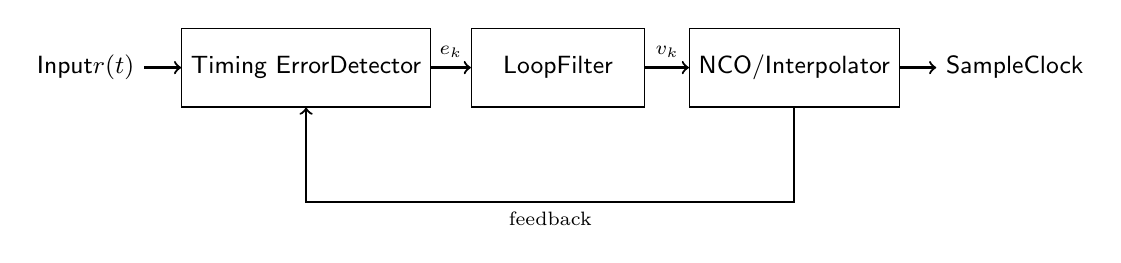
\begin{tikzpicture}[
  block/.style={rectangle, draw, minimum width=2.2cm, minimum height=1cm, font=\sffamily\small},
  node distance=2.5cm,
  font=\small
]
\node (input) {\sffamily Input\\$r(t)$};
\node[block, right of=input, node distance=2.8cm] (ted) {Timing Error\\Detector};
\node[block, right of=ted, node distance=3.2cm] (lf) {Loop\\Filter};
\node[block, right of=lf, node distance=3cm] (nco) {NCO/\\Interpolator};
\node[right of=nco, node distance=2.8cm] (output) {\sffamily Sample\\Clock};

% Forward path
\draw[->,thick] (input) -- (ted);
\draw[->,thick] (ted) -- node[above] {\scriptsize $e_k$} (lf);
\draw[->,thick] (lf) -- node[above] {\scriptsize $v_k$} (nco);
\draw[->,thick] (nco) -- (output);

% Feedback path
\draw[->,thick] (nco.south) -- ++(0,-1.2) -| node[near start, below] {\scriptsize feedback} (ted.south);
\end{tikzpicture}
\end{center}

\textbf{Components:}
\begin{itemize}
\item \textbf{Timing error detector:} Gardner, early-late, or ML algorithm
\item \textbf{Loop filter:} PI controller for stability
\item \textbf{NCO:} Numerically controlled oscillator adjusts sampling phase
\item \textbf{Interpolator:} Polyphase filter provides fractional delay
\end{itemize}

\section{Frame Synchronization}

\subsection{Purpose}

Frame synchronization identifies the start of packets/frames in a continuous symbol stream.

\textbf{Required for:}
\begin{itemize}
\item Header decoding (packet length, modulation/coding scheme)
\item Payload extraction
\item Retransmission protocols (ARQ)
\item Multiple access coordination
\end{itemize}

Without frame sync, the receiver cannot determine where one packet ends and another begins.

\subsection{Preamble Detection}

Transmit a known pattern (preamble) at the start of each frame.

\textbf{Correlation-based detection:}
\begin{equation}
C[n] = \sum_{k=0}^{L-1} r[n+k] \cdot p[k]^*
\end{equation}
where:
\begin{itemize}
\item $C[n]$ = correlation metric at time $n$
\item $r[n]$ = received signal sample $n$
\item $p[k]$ = known preamble pattern (length $L$)
\end{itemize}

\textbf{Detection threshold:}
\begin{equation}
|C[n]| > \gamma \quad \Rightarrow \quad \text{Frame detected at time } n
\end{equation}
where:
\begin{itemize}
\item $\gamma$ = detection threshold
\end{itemize}

The threshold $\gamma$ balances:
\begin{itemize}
\item \textbf{False alarm probability:} Detecting frame when none exists
\item \textbf{Missed detection probability:} Missing actual frame start
\end{itemize}

\subsection{Auto-Correlation Method}

WiFi and other systems use repeated preamble patterns for self-correlation.

\textbf{Example: WiFi 802.11a short preamble}---16-sample pattern repeated 10 times.

\textbf{Auto-correlation detector:}
\begin{equation}
R[n] = \sum_{k=0}^{15} r[n+k] \cdot r[n+k-16]^*
\end{equation}
where:
\begin{itemize}
\item $R[n]$ = auto-correlation at time $n$
\item 16 = repetition period (samples)
\end{itemize}

When the received signal aligns with the repetition pattern, $|R[n]|$ peaks, indicating frame start.

\textbf{Advantages:}
\begin{itemize}
\item[\checkmark] No stored template required (self-synchronizing)
\item[\checkmark] Robust to frequency offset
\item[\checkmark] Simultaneous frame detection and coarse CFO estimation
\end{itemize}

\subsection{Barker Codes}

Barker codes are binary sequences with ideal autocorrelation properties.

\textbf{11-bit Barker sequence:}
\begin{equation}
\{+1, +1, +1, -1, -1, -1, +1, -1, -1, +1, -1\}
\end{equation}

\textbf{Autocorrelation properties:}
\begin{itemize}
\item Peak value: 11 (at zero lag)
\item Sidelobe values: $\leq 1$ (at all other lags)
\end{itemize}

This provides excellent discrimination for frame detection in noisy environments.

\textbf{Application:} IEEE 802.11b (1--2~Mbps DSSS mode) uses 11-bit Barker coding for robust packet detection.

\subsection{Frame Structure: WiFi 802.11a Example}

\begin{center}
\begin{tikzpicture}[
  block/.style={rectangle, draw, minimum height=1.2cm, font=\sffamily\scriptsize},
  font=\scriptsize
]
% Frame components
\node[block, minimum width=2.5cm] (short) {Short\\Preamble\\8~$\mu$s};
\node[block, minimum width=2.5cm, right=0 of short] (long) {Long\\Preamble\\8~$\mu$s};
\node[block, minimum width=1.5cm, right=0 of long] (signal) {SIGNAL\\4~$\mu$s};
\node[block, minimum width=3cm, right=0 of signal] (data) {DATA\\(variable)};

% Annotations
\node[below=0.5cm of short, align=center] {\tiny AGC settling\\CFO coarse ($\pm 100$~kHz)\\Frame detection};
\node[below=0.5cm of long, align=center] {\tiny CFO fine ($\pm 1$~kHz)\\Channel estimation\\Timing sync};
\node[below=0.5cm of signal, align=center] {\tiny Rate\\Length\\Coding};
\node[below=0.5cm of data, align=center] {\tiny User payload};
\end{tikzpicture}
\end{center}

\textbf{Short preamble (8~$\mu$s):}
\begin{itemize}
\item 10$\times$ repetition of 1.6~$\mu$s pattern (16 samples)
\item Functions: AGC settling, coarse CFO ($\pm 100$~kHz range), frame detection
\end{itemize}

\textbf{Long preamble (8~$\mu$s):}
\begin{itemize}
\item 2$\times$ known OFDM symbols (3.2~$\mu$s each)
\item Functions: Fine CFO ($\pm 1$~kHz accuracy), channel estimation (64 subcarriers), symbol timing
\end{itemize}

\textbf{Total sync overhead:} 16~$\mu$s per packet.

\section{Applications}

\subsection{GPS L1 C/A Acquisition}

GPS presents an extreme synchronization challenge: signal power is $-130$~dBm, \textbf{below the noise floor}.

\textbf{System parameters:}
\begin{itemize}
\item \textbf{C/A code:} 1023-chip Gold code at 1.023~MHz (1~ms period)
\item \textbf{Doppler range:} $\pm 5$~kHz (satellite motion)
\item \textbf{Processing gain:} 30~dB from spreading
\end{itemize}

\textbf{Acquisition process:}
\begin{enumerate}
\item \textbf{2D search:} Doppler frequency ($\pm 5$~kHz) and code phase (0--1023 chips)
\item \textbf{FFT-based correlation:} Fast frequency-domain processing
\item \textbf{Integration:} Accumulate multiple code periods
\item \textbf{Threshold detection:} Declare acquisition when SNR $> 10$~dB post-correlation
\end{enumerate}

\textbf{Acquisition time:}
\begin{itemize}
\item Cold start (no almanac): 0.1--1~second
\item Hot start (known satellite positions): 1--10~ms
\end{itemize}

\subsection{LTE Cell Search}

LTE uses hierarchical synchronization signals for initial cell acquisition.

\textbf{Primary Synchronization Signal (PSS):}
\begin{itemize}
\item 3 Zadoff-Chu sequences (each represents one of 3 sector IDs)
\item Transmitted every 0.5~ms (slot boundary)
\item Functions: Slot timing, initial frequency offset, sector ID
\end{itemize}

\textbf{Secondary Synchronization Signal (SSS):}
\begin{itemize}
\item 168 possible sequences (2 sequences per cell group)
\item Determines frame timing and full cell ID (504 unique cells)
\end{itemize}

\textbf{Cell search procedure:}
\begin{enumerate}
\item \textbf{PSS detection:} Correlate with 3 possible sequences every 0.5~ms
\item \textbf{Coarse CFO estimation:} From PSS phase progression
\item \textbf{SSS detection:} Identify one of 168 sequence pairs
\item \textbf{Fine CFO estimation:} From SSS phase
\item \textbf{PBCH decode:} Master Information Block (system bandwidth, frame number)
\end{enumerate}

\textbf{Cell search time:}
\begin{itemize}
\item Initial acquisition: $\sim 100$~ms
\item Handover (known neighbor): $\sim 10$~ms
\end{itemize}

\subsection{DVB-S2 Satellite Receiver}

Satellite links have large frequency offsets due to Doppler shift and local oscillator drift.

\textbf{Synchronization challenges:}
\begin{itemize}
\item \textbf{Coarse CFO:} $\pm 500$~kHz (Doppler from satellite motion + LNB drift)
\item \textbf{Timing offset:} $\pm 100$~ppm (clock mismatch)
\item \textbf{Low SNR:} Typical $E_b/N_0 = 5$--10~dB
\end{itemize}

\textbf{Acquisition sequence:}
\begin{enumerate}
\item \textbf{PLHEADER detection:} 90-symbol pilot block marks frame start
\item \textbf{Coarse timing:} Sliding correlation over uncertainty window
\item \textbf{Fine CFO/phase:} Pilot symbols inserted every 16 data symbols
\item \textbf{Tracking:} Decision-directed feedback using decoded data
\end{enumerate}

\textbf{Acquisition time:}
\begin{itemize}
\item Blind frequency search: $\sim 1$~second
\item Known frequency: $\sim 100$~ms
\end{itemize}

\section{Performance Analysis}

\subsection{Impact of Synchronization Errors on BER}

Synchronization errors directly degrade bit error rate performance.

\subsubsection{CFO Impact on Constellation}

Small normalized CFO ($\epsilon = 0.01$):
\begin{equation}
\phi_{\text{rotation}} = 2\pi \epsilon \cdot n = 0.0628n \text{ radians/symbol}
\end{equation}

After 10 symbols: $\phi = 0.628$ radians $\approx 36°$.

\textbf{Result:}
\begin{itemize}
\item QPSK: Acceptable ($\pm 45°$ tolerance)
\item 256-QAM: \textbf{Fails} ($\pm 2.8°$ tolerance exceeded)
\end{itemize}

Large CFO ($\epsilon = 0.2$) in OFDM causes severe ICI, resulting in $>10$~dB SNR loss.

\subsubsection{Phase Noise Effects}

Oscillator phase jitter modeled as Gaussian:
\begin{equation}
\phi_n[k] \sim \mathcal{N}(0, \sigma_\phi^2)
\end{equation}
where:
\begin{itemize}
\item $\phi_n[k]$ = phase noise at symbol $k$
\item $\sigma_\phi$ = RMS phase error (radians)
\end{itemize}

\textbf{Phase noise tolerance by modulation:}

\begin{center}
\begin{tabular}{@{}lr@{}}
\toprule
\textbf{Modulation} & \textbf{RMS Phase Tolerance} \\
\midrule
QPSK & $\sim 10°$ \\
16-QAM & $\sim 5°$ \\
64-QAM & $\sim 2°$ \\
256-QAM & $\sim 1°$ \\
1024-QAM & $\sim 0.5°$ \\
\bottomrule
\end{tabular}
\end{center}

\subsubsection{Timing Jitter Impact}

Clock instability causes sampling time variation. Effective SNR degradation:
\begin{equation}
\text{SNR}_{\text{eff}} = \text{SNR} \cdot \text{sinc}^2(\pi \sigma_\tau)
\end{equation}
where:
\begin{itemize}
\item $\sigma_\tau$ = RMS timing error (fraction of symbol period)
\end{itemize}

\textbf{Example:} $\sigma_\tau = 0.1$ results in 0.4~dB SNR loss.

\section{Worked Example: WiFi 802.11n Synchronization}

\textbf{Scenario:} Design synchronization for WiFi 802.11n receiver at 2.4~GHz.

\subsection*{Given Parameters}

\begin{tabular}{@{}ll@{}}
Carrier frequency & $f_c = 2.437$~GHz (channel 6) \\
Crystal tolerance & $\pm 20$~ppm \\
OFDM subcarrier spacing & $\Delta f = 312.5$~kHz \\
Symbol rate & $R_s = 250$~ksps (per subcarrier) \\
Modulation & 64-QAM \\
Required BER & $10^{-5}$ \\
\end{tabular}

\subsection*{Step 1: Calculate Maximum CFO}

\begin{equation}
\Delta f_{\max} = f_c \times \text{tolerance} \times 2
\end{equation}
\begin{equation}
\Delta f_{\max} = 2.437 \times 10^9 \times 20 \times 10^{-6} \times 2 = 97.5 \text{ kHz}
\end{equation}

Factor of 2 accounts for TX and RX oscillator errors combining.

\subsection*{Step 2: Calculate Normalized CFO}

\begin{equation}
\epsilon_{\max} = \frac{\Delta f_{\max}}{R_s} = \frac{97{,}500}{250{,}000} = 0.39
\end{equation}

This is 39\% of symbol rate---\textbf{severely degrading without correction}.

\subsection*{Step 3: Phase Error Tolerance for 64-QAM}

64-QAM constellation has 8 points per axis, angular spacing:
\begin{equation}
\Delta\phi_{\text{decision}} = \frac{360°}{64} = 5.625°
\end{equation}

Safe margin: $\pm 2°$ RMS phase error.

\subsection*{Step 4: Timing Error Tolerance}

For negligible BER degradation ($< 0.5$~dB loss):
\begin{equation}
\sigma_\tau < 0.1T \quad \text{(10\% of symbol period)}
\end{equation}

\subsection*{Step 5: Synchronization Strategy}

\textbf{Two-stage acquisition:}
\begin{enumerate}
\item \textbf{Coarse CFO (short preamble):} Auto-correlation, range $\pm 100$~kHz
\item \textbf{Fine CFO (long preamble):} Cross-correlation, accuracy $\pm 1$~kHz
\item \textbf{Phase tracking:} Decision-directed, loop BW $= 0.02 R_s = 5$~kHz
\item \textbf{Timing recovery:} Gardner detector, loop BW $= 0.01 R_s = 2.5$~kHz
\end{enumerate}

\begin{calloutbox}[colback=black!8!white,colframe=black]{Synchronization Budget}
\textbf{Result: System meets 64-QAM requirements}

Residual errors after sync:
\begin{itemize}
\item CFO: $< 1$~kHz ($\epsilon = 0.004$) $\rightarrow$ $< 1.5°$ rotation per symbol
\item Phase error: $< 1.5°$ RMS (pilot-aided tracking)
\item Timing error: $< 0.08T$ (Gardner detector)
\end{itemize}

\textbf{Conclusion:} Synchronization overhead (16~$\mu$s preamble) enables reliable 64-QAM operation in 20~ppm crystal environment.
\end{calloutbox}

\section{Summary}

\begin{center}
\begin{tabular}{@{}ll@{}}
\toprule
\textbf{Synchronization Type} & \textbf{Key Characteristics} \\
\midrule
Carrier frequency & Range: $\pm 20$--50~ppm typical \\
                  & Methods: Preamble correlation, blind \\
Carrier phase     & Tolerance: $\pm 90°$ (BPSK) to $\pm 2.8°$ (256-QAM) \\
                  & Methods: PLL, Costas loop, decision-directed \\
Symbol timing     & Tolerance: $< 0.1T$ for negligible loss \\
                  & Methods: Early-late, Gardner, ML \\
Frame sync        & Detection: Correlation with preamble \\
                  & Sequences: Barker codes, Zadoff-Chu \\
\bottomrule
\end{tabular}
\end{center}

\textbf{Key trade-offs:}
\begin{itemize}
\item \textbf{Loop bandwidth:} Narrow (better noise rejection) vs wide (faster acquisition)
\item \textbf{Preamble length:} Short (low overhead) vs long (better accuracy)
\item \textbf{Pilot density:} Sparse (low overhead) vs dense (better tracking)
\end{itemize}

\textbf{Typical synchronization times:}
\begin{itemize}
\item WiFi packet: 16~$\mu$s
\item LTE cell search: 100~ms (cold start)
\item GPS acquisition: 0.1--1~second
\item Satellite (DVB-S2): 1~second (blind)
\end{itemize}

\section{Further Reading}

\begin{itemize}
\item \textbf{Chapter~\ref{ch:bpsk}:} Binary Phase-Shift Keying---carrier recovery for PSK
\item \textbf{Chapter~\ref{ch:qpsk}:} QPSK Modulation---phase synchronization requirements
\item \textbf{Signal Chain:} End-to-end processing flow including sync
\item \textbf{Channel Equalization:} Frequency-selective fading correction
\item \textbf{OFDM:} Pilot-based synchronization in multicarrier systems
\item \textbf{Bit Error Rate:} Performance degradation with sync errors
\end{itemize}
